%%%%%%%%%%%%%%%%%%%%%%%%%%%%%%%%%%%%%%%%%%%%%%%%%%%%%%%%%%
%
% Vzor pro sazbu kvalifikační práce
%
% Západočeská univerzita v Plzni
% Fakulta aplikovaných věd
% Katedra informatiky a výpočetní techniky
%
% Petr Lobaz, lobaz@kiv.zcu.cz, 2016/03/14
%
%%%%%%%%%%%%%%%%%%%%%%%%%%%%%%%%%%%%%%%%%%%%%%%%%%%%%%%%%%

% Možné jazyky práce: czech, english
% Možné typy práce: BP (bakalářská), DP (diplomová)
\documentclass[czech,DP]{thesiskiv}

% Definujte údaje pro vstupní strany
%
% Jméno a příjmení; kvůli textu prohlášení určete, 
% zda jde o mužské, nebo ženské jméno.
\author{Kateřina Kratochvílová}
\declarationfemale

%alternativa: 
%\declarationfemale

% Název práce
\title{Nástroj pro automatickou identifikaci KIR alel}

\thanktext{Ráda bych poděkovala Ing. Lucii Houdové, Ph.D. za cenné rady, věcné připomínky, trpělivost a ochotu, kterou mi v průběhu zpracování této práce věnovala.}
% 
% Texty abstraktů (anglicky, česky)
%
\abstracttexten{The text of the abstract (in English). It contains the English translation of the thesis title and a short description of the thesis.}

\abstracttextcz{Text abstraktu (česky). Obsahuje krátkou anotaci (cca 10 řádek) v češtině. Budete ji potřebovat i při vyplňování údajů o bakalářské práci ve STAGu. Český i anglický abstrakt by měly být na stejné stránce a měly by si obsahem co možná nejvíce odpovídat (samozřejmě není možný doslovný překlad!).
}

% Na titulní stranu a do textu prohlášení se automaticky vkládá 
% aktuální rok, resp. datum. Můžete je změnit:
%\titlepageyear{2016}
%\declarationdate{1. března 2016}

% Ve zvláštních případech je možné ovlivnit i ostatní texty:
%
%\university{Západočeská univerzita v Plzni}
%\faculty{Fakulta aplikovaných věd}
%\department{Katedra informatiky a výpočetní techniky}
%\subject{Bakalářská práce}
%\titlepagetown{Plzeň}
%\declarationtown{Plzni}

%%%%%%%%%%%%%%%%%%%%%%%%%%%%%%%%%%%%%%%%%%%%%%%%%%%%%%%%%%
%
% DODATEČNÉ BALÍČKY PRO SAZBU
% Jejich užívání či neužívání záleží na libovůli autora 
% práce
%
%%%%%%%%%%%%%%%%%%%%%%%%%%%%%%%%%%%%%%%%%%%%%%%%%%%%%%%%%%

% Zařadit literaturu do obsahu
\usepackage[nottoc,notlot,notlof]{tocbibind}

% Umožňuje vkládání obrázků
\usepackage[pdftex]{graphicx}

% Odkazy v PDF jsou aktivní; navíc se automaticky vkládá
% balíček 'url', který umožňuje např. dělení slov
% uvnitř URL
\usepackage[pdftex]{hyperref}
\hypersetup{colorlinks=true,
  unicode=true,
  linkcolor=black,
  citecolor=black,
  urlcolor=black,
  bookmarksopen=true}

\usepackage{float}

% Při používání citačního stylu csplainnatkiv
% (odvozen z csplainnat, http://repo.or.cz/w/csplainnat.git)
% lze snadno modifikovat vzhled citací v textu
\usepackage[numbers,sort&compress]{natbib}

%%%%%%%%%%%%%%%%%%%%%%%%%%%%%%%%%%%%%%%%%%%%%%%%%%%%%%%%%%
%
% VLASTNÍ TEXT PRÁCE
%
%%%%%%%%%%%%%%%%%%%%%%%%%%%%%%%%%%%%%%%%%%%%%%%%%%%%%%%%%%
\begin{document}
%
\maketitle
\tableofcontents

\chapter{Úvod}



\section{Bordel}
Její podstata spočívá v tom, že si organismus uchová část B lymfocytů (tzv. paměťový T-lymfocyt, viz imunologická paměť), které jsou odpovědné za výrobu specifických protilátek proti patřičnému patogenu. Organismus tak může spustit specifickou imunitní odpověď okamžitě a masově po zaznamenání infekce, aniž by předtím musel složitě hledat vhodné buňky k produkci patřičných protilátek. Právě této vlastnosti využívá očkování.



\chapter{Geny}
V každé buňce lidského organismu, konkrétně v buněčném jádře, je možné nálest 46 chromozomů. Jeden chromozom představuje stočenou dlouhou molekulu DNA (Deoxyribonuklenovou kyselinu). Všech 46 chromozomů obsahuje okolo 100 000 genů. Drobný segment DNA, který řídí buněčnou funkci je právě gen. Konkrétní forma genu je alela. \citep{en_smith} Uvnitř buňky máme celý genom který se ovšem nemusí projevit na povrchu buňky. Pokud se vlastnost kterou gen přenáší projeví na povrchu buňky označujeme to jako exprese genu (jeho sebevyjádření).


\section{Imunitní systém aneb kde se vzal KIR}
Imunitní systém chrání organismus před škodlivinami. Skládá se ze dvou hlavních částí vrozené imunity a získané imunity. 

\subsection{Vrozená imunita}
Vrozená imunita též označována přirozená, neadaptivní, antigenně nespecifická je neměnně zapsána v DNA. To znamená, že při každém setkání s antigenem odpoví stejnou reakcí. Buňky nesoucí vrozenou imunitu jsou stále přítomně v krvy, takže jejich případná aktivace je takřka okamžitá (minuty až hodiny). Do této imunity patří i natural killer buňky s KIR receptory, které budou dále rozebírány v textu. 

\subsection{Získaná imunita}
Získaná imunita též označována specifická či adaptivní oproti specifické má v genomu zapsány pouze své základy. V průběhu lidského života se vyvyjí a mění. Změna může nastat například očkování nebo proděláním patřičné choroby, může být ale dočasná. Z těchto důvodů může být odpověď ziskáné imunity při setkání se stejnou chorobou rozdílná. Fungování získané imunity zajišťují T- a B- lymfocyty, ale nefunguje samostantně. Při zabíjení patogenů spolupracuje s vrozenou imunitou.

\subsection{Antigen}
Antigenem označujeme látky, které imunitní systém rozpozná a zareaguje na ně. Nejčastější antigeny jsou cizorodé látky z vnějšího prostředí.






\section{Imunitní systém, HLA a non-HLA geny}
Human leucocyte antigen(HLA) je genetický systém, který je primárně zodpovědný za rozeznávání vlastního od cizorodého. Tento systém je složen právě z jednotlivých HLA genů, které následně svojí expresí na povrch buňky do HLA molekul rozpoznávají antigeny (cizorodé částice). Pokud HLA molekula přijde do styku s antigenem je antigen zničen.

HLA obsahuje pravděpodovně i geny odpovědné za intenzitu imunitní odpovědi.


HLA antigeny je skupina bílkovin, jsou lokalizovány na povrchu buněk klíčové pro imunitní systém.
Zjednodušeně lze říci že HLA molekuly, imunoglobuliny a receptory T-lymfocytů jsou základem adaptivní imunity člověka

HLA je rozsáhlý komplex genů, které determinují (určují, rozpoznávjí????) povrchové molekuly (antigeny) umístěné v plazmatické membráně buněk

Hlavní fyziologickou funkcí molekul MHC je předkládat antigeny nebo jejich fragmenty buňkám imunitního systému, především T-lymfocytům (prezentace antigenu je prvním předpokladem pro rozvoj imunitní reakce a tím obrany proti napadení mikroorganismy). Pomocí těchto molekul buňky imunitního systému vzájemně kooperují.

Non-HLA geny jsou geny které se nepodílejí na základní funkci HLA systému.
\\základní rozdíl mezi HLA a non-HLA a kir

Non-HLA geny jsou geny které se nepodílejí na základní funkci HLA systému. Z III třídy jsou to všechny, z II žádný a z I je to směs. Zjednodušeně můžeme říci, že geny které nejsou HLA jsou non-HLA. Tyto geny souvisejí též s funkcí imunitního systému, ne však vylučně s funkcí HLA. 


někdy je termín HLA a MHC zaměňován.. MHC je tedy souhrný termín pro všechny komplexy kdy podskupinou jsou HLA jen pro lidi a stejně tak může být DLA který je jen pro psy.. 
Z funkčního i biologického hlediska jde však u všech savců o stejnou skinu genů

Ze strukturárního hlediska je možné HLA geny rozdělit do 2 základních skupin HLA I a II třídy.




Mezi těmito 2 regiony se nachází region III (někdy
označován jako region HLA III. třídy) s geny pro komplement
(C4), některé cytokiny (TNF alfa) a stresové proteiny (hsp). Zatímco
16prakticky všechny geny regionu II se nějakým způsobem podílí na
základní funkci HLA systému - tj. zpracování a prezentaci
antigenů T-lymfocytům, z genů regionu III žádný a region třídy I je
v tomto směru intermediární, tj. obsahuje směs genů jak
bezprostředně se podílejících, tak přímo nesouvisejících s funkcí
HLA systému.

V HLA I je přibližně 20 genů hlavní jsou HLA- A, -B a -C
další jsou HLA E, F, G, MICA a MICB
Další geny – HLA H, J, K a MICC- jsoupseudogeny.

HLA II HLA
DR, HLA DP as HLA DQ.
pak ještě DM, DO

Diverzita genů vznikla na díky nepřetržité snaze učině eliminovat neustále se měnící spektrum patogenů.

Z hlediska dědičnosti jsou všechny geny kódující HLA molekuly
kodominantní a řídí se mendelovským typem dědičnosti. Všechny
geny HLA systému na 6. chromozómu se dědí vcelku jako blok –
takzvaný haplotyp. Jedinci jsou heterozygotní a mají tak na
buňkách dvě kompletní sady HLA antigenů.
Geny HLA systému vykazují poměrně těsnou genetickou vazbu
takže se většinou přenášejí jako bloky genů, mezi kterými pouze
výjimečně dochází k rekombinaci (crossing-over). Rodinné studie
ukázaly, že pro některé regiony uvnitř HLA komplexu je relativní
absence rekombinací („crossing-over“) obzvláště typická. Jde
především o subregiony HLA-B k HLA-C a HLA-DQB1 k HLA-
DRB1. Tyto regiony jsou někdy označovány jako „polymorfní
zmražené bloky“ a jejich odolnost vůči rekombinacím je základem
vazebné nerovnováhy (linkage disequilibrium) – tedy nenáhodné
asociaci alel 2 nebo více lokusů- mezi specifickými alelami HLA-
B a HLA-C, respektive HLA-DR a DQ.
Populačně genetické studie prokázaly, že vazebná nerovnováha
je dokonce typickým rysem HLA systému. Mezi pravděpodobné
příčiny patří již uváděná redukovaná frekvence rekombinací a
selekce ve prospěch vázaného polymorfismu (18), podrobnější
rozbor by byl nad rámec textu. Ukázkovým příkladem této
vazebné nerovnováhy je nejčastější indoevropský („kavkazoidní“)
haplotyp A1-B8-DR3, který se v bělošské populaci vykytuje až
s 5-10% frekvencí a někdy je nazýván ancestrálním haplotypem
AH8.1 (viz též dále 1.1.8).

\subsection{Jak vypadá genom} 
Genová oblast HLA komplexu, se nalézá na krátkem raménku 6. chromozomu (6p21.31), zaujímá úsek dlouhý 3600 kb
(3,6cM), tedy přibliţně jednu tisícinu genomu. Obsahuje 224 genů; 128 funkčních genů
a 96 pseudogenů a patří k regionům s nejvyšší genovou hustotou.

Uprostřed HLA oblasti se nachází úsek o velikosti 1 Mb, ve kterém bylo identifikováno na
70 genů, které se funkčně ani strukturně nepodobají HLA molekulám. Navzdory této
skutečnosti se vžilo označení geny III. třídy, přičemž některé geny původně zařazené do
této třídy jsou nověji označovány jako geny IV. třídy (viz. výše).

HLA-6.Chromozom a KIR 19.chromozom
udíž se segregují nezávisle a
HLA shodní dárci s příjemce mají obvykle různé složení KIR genů (Fryčová)


\section{10/10}
Ta je postavena na případě typizace 5 lokusů (HLA-A/B/C/DRB1/ /DQB1). Vstupním parametrem samotného vyhledávání je míra shody (match) či definované neshody (mismatch). Navržená metoda je platná nejen pro úplnou míru shody 10/10 (shoda HLA-A/B/C/DRB1/DQB1), ale i menší, např. 8/8 (HLA-A/B/C/DRB1), či požadovanou neshodu na konkrétních lokusech, např. 9/10 HLA-A mismatch. 

Během vyhledávání se hodnotí shoda obou alel v lokusech HLA-A, HLA-B, HLA-C,
HLA-DRB1 a HLA-DQB1. Cílem je najít dárce, který bude s příjemcem shodný v 10 znacích
z 10. V závislosti na pacientově stavu a nízké pravděpodobnosti najít včas shodného
nepříbuzného dárce je možné tolerovat odchylky v jednom nebo dvou znacích (9/10,
8/10). Každá odchylka však zvyšuje riziko rozvoje potransplantačních komplikací.
\\
dědičnost HLA znaků
\\
Každý člověk má tzv. fenotyp neboli soubor HLA znaků, který je složen právě
ze dvou haplotypů. Každý z haplotypů je tvořen sadou antigenů obsahujících konkrétní
alely. Polovinu těchto znaků zdědíme od matky a polovinu od otce.
Z hlediska transplantace se v současné době považují za nejdůležitější (a proto
se také nejpřesněji vyšetřují) HLA antigeny I. třídy A, B, C a antigeny II. třídy DR a
DQ. Existuje ale řada dalších – tzv. minoritních antigenů, které dosud nejsou
dostatečně probádány, a jejich vliv na průběh transplantace se teprve zkoumá.
V současnosti je požadavek na míru shody 10/10 neboli v pěti HLA antigenech,
konkrétně v (HLA -A, -B, -C, -DRB1 a –DQB1). Nejmenší možná shoda představuje
6/10 v genech (HLA -A, -B, -DRB1), ale zde bohužel pro pacienta vzniká smrtelné
riziko odvržení štěpu.
\\
\\
Počet teoreticky možných kombinací HLA znaků u člověka dosahuje několika
miliard. Je známo, že některé tkáňové typy (kombinace znaků) se vyskytují v určitém
národě či oblasti častěji, jiné jsou extrémně vzácné. Protože se jednotlivé znaky dědí,
shodu mezi dvěma jedinci najdeme nejsnáze v pokrevním příbuzenstvu. Od rodičů na
potomky se příslušná polovina znaků předává obvykle ve zmíněné kompletní sadě
(haplotypu).
Pro zjednodušení je uveden příklad, podle kterého je dle genetických zákonů
možné dědit jednu ze čtyř možných variant výše zmíněných druhů HLA antigenů mezi
sourozenci (obr. 3.2).

\section{Porovnání vhodného dárce}
V případě nepříbuzenských transplantací se vybírají potenciální dárci, kteří nemají s daným
pacientem žádný děděný haplotyp. Snahou je najít takového dárce, který má shodné, přestože
děděné od jiných rodičů, HLA antigeny. Informace o tom, jak jsou alely haplotypicky
uspořádány obvykle chybí, proto je vždy nutná typizace maximálním rozlišením ve více
HLA lokusech. Zjišťovaný minimální rozsah HLA shody se v jednotlivých transplantačních
centrech liší. V současné době je u nepříbuzného páru požadována typizace vysokým
rozlišením v lokusech HLA – A, B, C, DR a DQ (http://www.efiweb.eu/efi-
committees/standards-committee.html). Pokud pacient a dárce mají stejné alely na všech
těchto lokusech, hovoříme o shodě 10/10. Při jedné neshodě se jedná o shodu 9/10, při dvou o
shodu 8/10.
K typizaci se nejčastěji používá PCR – SSP (PCR se sekvenačně specifickými primery) či
SBT (sequence based typing) technika, v posledních letech se stává zlatým standardem přímá
sekvenace (SBT) HLA genu.
fričová
U HLA - A, B, C, DR a DQ požaduje se typizace v těchto lokusech. Pokud má dárce shodu ve všechn lokusech hovoříme o shodě 10/10 při jedné neshodě je to 9/10.
\\

\section{Natural Killer a KIR}
Mezi rizika při transplantaci krvetvorných buněk patří reakce štěpu proti hostiteli nebo relaps oněmocnění (návrat nemoci). Podle nedávných studiích výsledky příjetí štěpu ovlivňují nejenom HLA geny ale i non-HLA geny. Jedním z nich může být právě killer immunoglobulin-like receptor (KIR). V případě kdy by bylo nalezeno více vhodných dárců, tj. se shodou 10/10 nebo 9/10, vybíralo by se následně podle KIR genů \cite{KIR_transplantace_jindra} \cite{Frycova_bakalarka}.

\subsection{Natural killer}
NK buňky (Natural killer) jsou velké granulární lymfocyty vrozeného imunitního systému. V krevním oběhu lidského těla je jich možné nalést $10-15\%$. 
\\
\\
Klíčovou vlastností NK buněk je nejenom schopnost rozlišit poškozené buňky od zdravích ale i poškozené buňky rychle a efektivně likvidovat. Poškozené buňky mohou být buňky infokované virem či buňky transfomované v nádorové. 

\subsection{KIR}
Killer immunoglobulin-like receptor (KIR) jsou receptory na povrchu NK buněk. Natural killer buňky oproti B- a T- lymfocitům (buňkám získané imunity) nemají antigenně specifické receptory. NK buňky rozpoznávají a zabíjejí buňky na základě interakce mezi KIR receptorem a HLA molekulou na povrchu zkoumané buňky. 
\\
\\
KIR receptory můžeme rozdělit na inhibiční a aktivační. Zda dojde k aktivaci NK buňky rozhoduje právě jejich rovnováha na zkoumané buňce. Zatímco inhibiční receptory se váží hlavně na molekuly HLA, aktivační receptory rozpoznávají molekuly které jsou exprimovány na membránu při buněčném stresu.
\\
\\
NK buňky ustavičně prohledávají své okolí a testují přítomnost příslušných HLA ligand (specifická HLA molekula) pro své KIR receptory. Pokud je příslušný HLA ligand přítomen naváže se na NK buňku (\ref{fig:kir_princip} případ~1). Tímto systémem jsou ochráněny vlastní HLA buňky. Pokud přítomen není je spuštěna cytotoxická reakce (schopnost níčit buňky) a zkoumaná buňka je zníčena.
\\
\\
Některé virem napadené buňky potlačují propsání HLA ligand na povrch buňky a tím se brání cytotoxicitě proti T lymfocitům, ale naopak jsou více citlivější na cytotoxicitu proti NK buňkám. Ukázano na obrázku \ref{fig:kir_princip} případ~3.
\begin{figure}[H]		
		\centering
		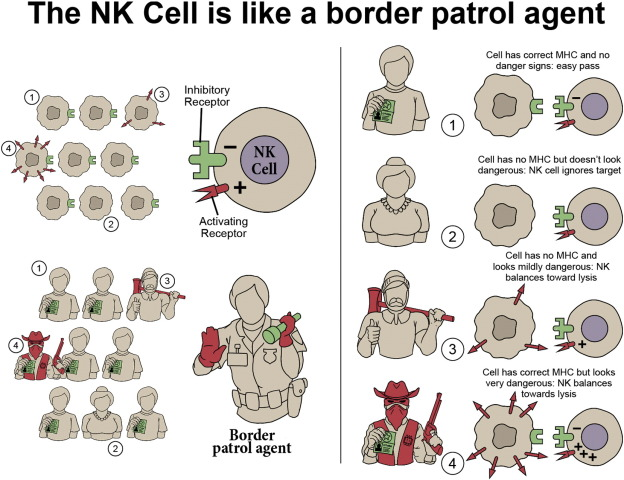
\includegraphics[width=\textwidth]{./img/NK_princip.jpg}
		\caption{Přirovnání fungování natural killer buňky k pasové kontrole \cite{KIR_img_princip}. V pravé části jsou zobrazené případy které mohou nastat když natural killer buňka potká jinou buňku. V prvním případě je tělu vlastní zdravá buňka, kde se KIR receptor naváže na HLA ligand a k cytotoxitické reakci nedojde. V druhém případě je červená krvinka k cytotoxicitě opět nedojde, protože na zkoumané buňce nepřevažují aktivační receptory. V 3 případě je to nádorová buňka, která schová HLA ligand (může nastat po transplantaci kostní dřeně) a tím se "schová" proti T- lymfocytům. Avšak aktivační receptory převládají a tak k cytotoxicitě dojde. Ve 4 příkladě je nádorová buňka nebo virem nakažená buňka (stresové ligandy). Aktivační receptory převládají k cytotoxicitě dojde.}
		\label{fig:kir_princip}
\end{figure}

V případě transplantace je jedním z možných řešení pacientovi dát štěp, který obsahuje aktivační KIR receptory, které nemají jeho buňky.

\subsection{Nomenklatura KIR genů}
KIR geny (na obrázku \ref{fig:img_kir_nomenklatura} se liší různou délkou cytoplasmatických ocásku (tail) a různým počtem imunoglobulin-like domén (lg-like). Na základě této rozmanitosti byla založena nomenklatura KIR genů, tedy jejich pojmenování. 
\\
\\
Jak je vidět na obrázku~\ref{fig:img_kir_nomenklatura}, cytoplasmatický ocásek může být dlouhý (long~-~L) nebo krátký (short~-~S). Oproti tomu imunoglubulínové domény se mohou vyskytovat 2~(2D) nebo 3~(3D). 

\begin{figure}[H]		
		\centering
		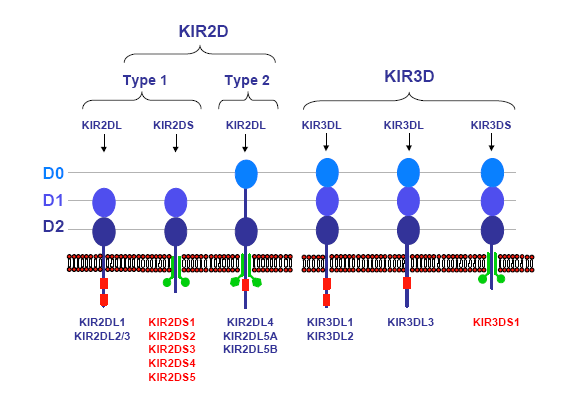
\includegraphics[width=\textwidth]{./img/KIR_nomenklatura.png}
		\caption{Nomenklatura KIR genů. \cite{KIR_transplantace_jindra}}
		\label{fig:img_kir_nomenklatura}
\end{figure}

Další rozdělení KIR genů je již výše zmíněné inhibiční a aktivační. Na obrázku~\ref{fig:img_kir_ligand} je možné si povšimnout detailu, že až na KIR2DL4 jsou aktivační KIR s krátkým ocáskem, zatímco inhibiční jsou s dlouhým ocáskem. Obrázek dále uvádí vazebné ligandy pro jednotlivé receptory. 
 
\begin{figure}[H]		
		\centering
		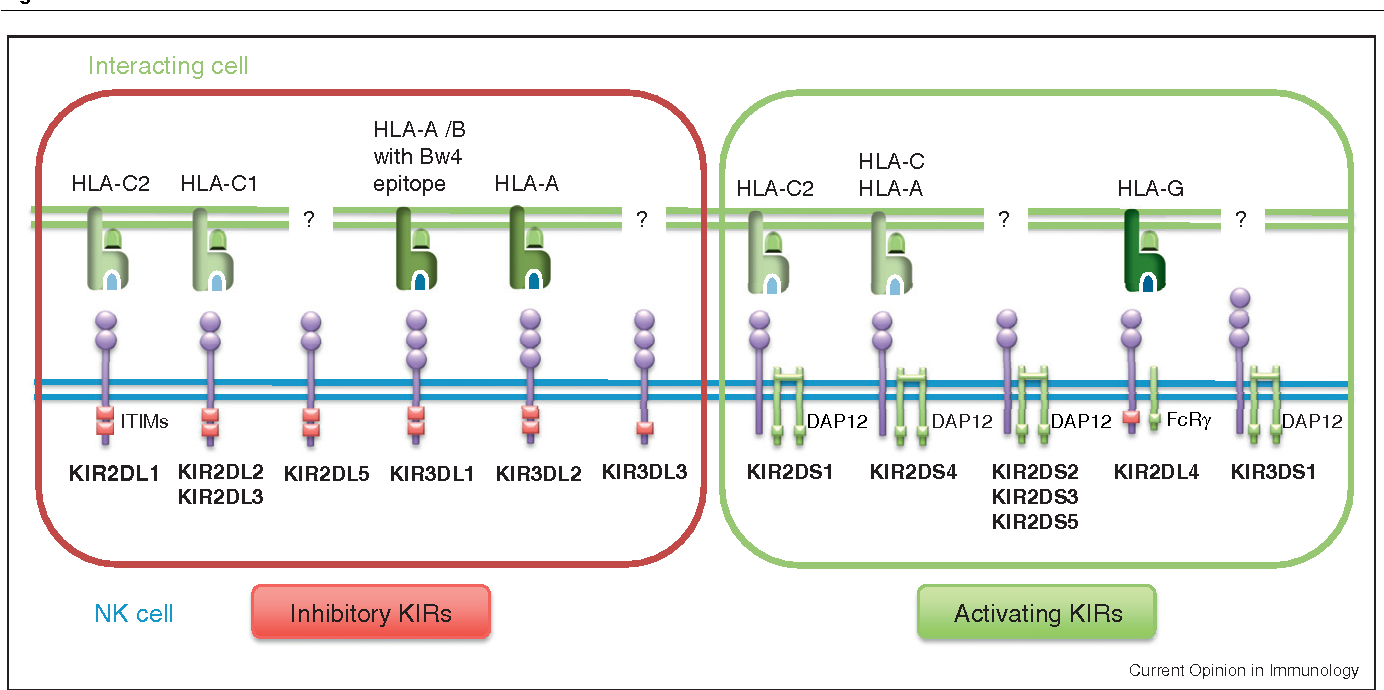
\includegraphics[width=\textwidth]{./img/KIR_nomenklatura2.png}
		\caption{KIR geny a jejich vazebné ligandy. Pokud je v obrázku ? značí to, že pro daný receptor neni znám vazebný ligand. \cite{KIR_img_nomenklatura}}
		\label{fig:img_kir_ligand}
\end{figure}




Bylo poprsáno celkem 15 exprimovaných KIR genů a 2 KIR pseudogeny


Pokud jde o vazebné partnery KIR (jejich ligandy), pak tyto jsou
známy především pro inhibiční receptory a ve všech případech jde o
HLA specificity I. třídy. Jedná se především o skupinu alel HLA-C alel
lišících se aminokyselinovým 
reziduem na pozicích
 77 a 80 $\alpha$
- helixu molekuly HLA-C (7). Byla publikována rozsáhlá data ukazující
10na význam inhibičních KIR a jejich HLA ligand pro výsledek
transplantace krvetvorných buněk

KIR geny/receptory a jejich vazební partneři (ligandy)
- fryčová ta tabulka tam byla zajímavá, stejná je i v tý disertačce od Jindry odtamtu to asi bude lepší
tak mě tak napadá jestli to A, B,C neni náhdou I, II, III.. protože píšou že se jedná hlavně o melekuly HLA C a non hla jsou všechn z III class.


KIR geny jsou lokalizovány na chromosomu 19q13.4 v oblasti zvané „leukocyte receptor
complex“ (LRC). Pro každý KIR gen navíc existují alelické varianty (Marsh et al, 2002;Hsu
et al, 2002). Tak jako geny HLA systému se i KIR geny dědí podobně a to jako celý blok
genů – haplotyp (viz obr. 3).

A je tam k tomu hezkej obrázek disertačka Jindra

Genetická diverzita KIR genů a genotypů připomíná diverzitu HLA
systému. Přestože jsou geny kódující KIR a HLA lokalizované na
různých chromozomech a segregují se tedy nezávisle, existují určité
důkazy alespoň částečné koevoluce obou systémů. Lze tudíž
předpokládat. U HLA restrihované populace lze tedy očekávat
alespoň částečnou redukci v diverzitě KIR genů i genotypů.
U HLA restrihované populace lze tedy očekávat
alespoň částečnou redukci v diverzitě KIR genů i genotypů.

Koevoluce je společný evoluční vývoj dvou či více druhů, při němž dochází k jejich vzájemnému přizpůsobování

Haplotypická variability KIR genů
KIR geny se vyskytují ve dvou hlavních haplotypech A a B, které jsou definovány typem a počtem specifických KIR genů.Ta je způsobena variabilitou v počtu a v typu
zastoupených KIR genů na daném haplotypu
Právě tato
haplotypická diverzita je hlavním důvodem populační diverzity KIR
genů a repertoáru NK buněk.
Neni žádné univerzální kriterium kteréé by je odlišovali

Skipina B je charakterizována přítomností alespoň jednoho nebo víze z následjících genů KIR2DL5, KIR2DS1, KIR2DS2, KIR2DS3, KIR2DS5 a KIR3DS1.

Skupina A je charakterizována absenzí těchto genů. 

Proto mají B více aktivačních KIR než A. A může mít jen KIR2DS4.

je tam obrázek zase u Jindry třeba.

U fryčoví jsem skončila na stránce 19. 
U jindry jsem skončila na stránce 14.





\section{bordel}
exprimovaný gen / pseudogeny
takže exprimovaný je ten který se propíše na povrch buňky a pseudogen je ten který se nepropíše na povrch buňky
Pseudogen je sekvence DNA, která je podobná genu, ale nedochází k jejímu přepisování v RNA (transkripci). Pseudogeny vznikají zpravidla určitou mutací, a to zejména v oblasti promotoru, regulační sekvence,[1] nebo sice RNA vzniká, ale je následně degradována.


NK buňky mají schopnost identifikovat molekuly vlastního MHC systému (Major
Histocompatilibity Compex), jmenovitě HLA I. třídy, které jsou normálně exprimovány
prakticky na všech buňkách v těle. Nádorové a některé virem napadené buňky potlačují
expresi HLA I. třídy a tím se brání napadení cytotoxickými T lymfocyty (Restifo, 1993).
Snížená exprese HLA I. třídy činí abnormální buňky citlivé k cytotoxicitě NK buněk (Karre,
1986). Molekuly HLA I. třídy rozpoznávají NK buňky pomocí pozitivních a negativních
13receptorů, které mohou inhibovat nebo naopak aktivovat NK buňky k „zabíjení“

Pokud to můžeme principálně zjednodušit, pak NK buňky neustále
systematicky „zkoumají“ přítomnost či absenci příslušných HLA
ligand pro své KIR receptory. Pokud je příslušný HLA ligand (HLA
molekula) přítomen, pak dojde k vazbě KIR-ligand HLA a jelikož za
normálních okolností vždy inhibiční KIR převládají nad aktivačními,
nedochází ke spuštění cytotoxické reakce NK buněk a takto jsou
„vlastní“ buňky chráněny před cytotoxicitou (viz část A a především D
na obr. 1). Pokud receptory KIR nenaleznou příslušný ligand HLA
(„vlastní“ molekulu HLA), nemůže být cytotoxicita příslušné NK buňky
prostřednictvím inhibičních receptorů KIR a náležitá cytotoxická
kaskáda je spuštěna


KIR jsou na povrchu NK buňek a kde jsou teda NK buňky? 
NK je v podstatě lymfocyt a to je typ bílé krvinky. jo a nebudou teda spíš  v lymfatické uzlině? 
leukocyty 1. granulocyty - neutrofilní, bazofilní a eozinogilní
		2. agranulocyty - lymfocyty a monocyty
		
neutrofilní granulocyty jsou schopny vycestovat z kapilár do místa zánětu
přeměněné monocyty přítomné v játrech v tělních dutinách (hrudní, bříšní), ve slezině vy lymfatických uzlinách a kostní dřeni

lymfocyty 
bílá krvinka je leukocyt
- typ bbílé krvinyky 
- T a B lymfocyty - specifická imunita
- NK buňky nespecifická imunita
- vznikají v z lymfatických kmenových buňek v kostní dřeni
Aha takže lymfatické řečiště je více propustné proto to co nejde do cév jde sem pak se to odfiltruje a pak se to vrací do krevního řečiště.

Velká buňka imunitního systému, nepotřebuje antigen aby začala zabíjet. 
-nespecifická imunita - vrozená, neadaptivní - veškeré potřebné informace zapsaná v DNA. Odpovídá při každém setkání s antigenem stejně - nemá paměť -> tady si to pročiřečí

Molekuly HLA I. třídy rozpoznávají NK buňky pomocí pozitivních a negativních receptorů, které mohou inhibovat nebo naopak aktivovat NK buňky k „zabíjení“

Tato schopnost destruovat cílové buňky je právě dána vzájemnou
interakcí mezi KIR receptory a příslušnou specifickou HLA molekulou
na povrchu buněk, neboli ligandem KIR receptorů
NK zabíjejí na základě interakce mezi KIR receptorem a HLA molekulou na povrchu buňky.
možná něco o inhibičních a aktivačních KIR 
\\
\\
NK buňky neustále systématicky testují přítomnost čí absenci příslušných HLA ligand pro své KIR receptory. Pokud je přítomen dojde k vazbě KIR-ligand HLA a nedojde k cytotoxické reakci (schopnost níčit buňky) , ochrana vlastních buněk. Pokud je 
nenajdou a je spuštěna cytotoxická kaskáda.
Některé virem napadané buňky nebo nádorové buňky potlačují expresi a tím se brání napadění cytotoxickými T lymfocyty
snížená exprese HLA I. třídy činí abnormální buňky cytlivé k cytotoxicitě NK buněk.

 Molekuly HLA I. třídy rozpoznávají NK buňky pomocí pozitivních a negativních
13receptorů, které mohou inhibovat nebo naopak aktivovat NK buňky k „zabíjení“

NK buňky maji shopnost identifikovat buňky vlastního MHC systému (HLA I.třídy) ktere jsou normálně exprimovány prakticky na všech buňkách v těle. 

V užším slova smyslu se jako ligand označuje signální molekula, která se váže na vazebné místo cílového proteinu. Ligand, který je schopný po navázání na receptor vyvolat fyziologickou odpověď, se nazývá agonista, ten, který je schopen se vázat, ale odpověď nespouští, je antagonista

Lze-li stručně shrnout, pak NK buňky s potenciálem iniciovat
cytotoxickou aloreakci používají KIRy jako inhibiční směrem k
„vlastním“, zdravým buňkám. Pokud však příslušný vlastní ligand
HLA na cílové buňce chybí, pak je iniciována cytotoxická reakce.
Celý tento koncept interakce KIR/HLA
a mechanismus regulace
cytotoxicity NK buněk se nazývá „missing-self“ hypotéza (3). Tím je
zaručena tolerance NK buněk k „vlastním“ a zdravým buňkám,
naopak alogenní („cizí“) buňky, či buňky s „down“- regulovanou HLA
molekulou (ligandem), což jsou typicky buňky nádorové či buňky
napadené virem, jsou efektivně eliminovány

Ligand je atom, ion nebo molekula, poskytující jeden nebo více elektronových párů centrálnímu atomu. Ligand je súčasťou komplexných (koordinačných) zlúčenín. Každá komplexná zlúčenina obsahuje centrálny atóm (katión) a anión alebo neutrálny komplex (ligand)
-wikiskripta
Ligand ve smyslu používaném v biochemii a farmakologii označuje látku, typicky malou molekulu, která vytváří komplex s biomolekulou a tato vazba má biologický význam. V užším slova smyslu se jako ligand označuje signální molekula, která se váže na vazebné místo cílového proteinu. Ligand, který je schopný po navázání na receptor vyvolat fyziologickou odpověď, se nazývá agonista, ten, který je schopen se vázat, ale odpověď nespouští, je antagonista
- wikipedie
Stručně lze shrnout, že NK buňky s potenciálem iniciovat cytotoxickou aloreakci používají
KIR receptory jako inhibiční, směrem k „vlastním“, zdravým buňkám. Pokud však příslušný
vlastní ligand HLA na cílové buňce chybí, pak dochází k iniciaci cytotoxické reakce. Proces
interakce KIR/HLA a mechanismus regulace cytotoxicity NK buněk se jako celek nazývá
14„missing-self“ hypotéza (Gasser a Raulet, 2006). Takto je zaručena tolerance NK buněk k
„vlastním“ a zdravým buňkám, naopak „cizí“ alogenní buňky, buňky s „down“ –
regulovaným
HLA ligandem (molekulou), což jsou typicky buňky napadené virem a
nádorové buňky, které jsou efektivně eliminovány

 Tato schopnost destruovat cílové buňky je dána
vzájemnou interakcí mezi KIR receptory a příslušnou specifickou
HLA molekulou na povrchu buněk, neboli ligandem KIR receptorů.

\subsection{Dědičnost KIR}
Jelikož jsou geny kódovány na různých chrmozomech (HLA 6 a KIR 19) takže HLA schodní dárci s příjemcem mají různé složení KIR genů.
KIR má dva haplotypy A a B .. a pak asi můžeš dělat kombinace AA, AB a BB.






Bylo zjištěno, že
specifické složení motivů centromerních a telomerních B haplotypů KIR genů přispívá
k ochraně před relapsem a zvyšuje šanci na úplné vyléčení AML.





\section{Jak funguje HLA}
\section{Jak funguje non-HLA}

\section{Bordel pro prvni kapitolu}
Takže to vypadá že nejdřív se najde shoda HLA a pak se ještě doděláváv KIR shoda.
Proč KIR? pOrotože roste počet důkazů vluvu genů KIR že mají vliv na výsledky transplance  při leukemii
HLA je na 6. chormozomu KIR je 19 chomozomu. tudiž se segregují nezávisle a Hla shodní dárci s příjemcem mají obvykle různé složení KIR genů
Nesmírná variabilita alel tohoto systému ztěžuje úspěšnost allogeních transplantací. 

\textbf{HLA}
jen zkopírováno a je ta i hezkej obrázek z %https://is.cuni.cz/webapps/zzp/detail/49783?lang=en
Genová oblast HLA komplexu, se nalézá na krátkem raménku 6. chromozomu (6p21.31), zaujímá úsek dlouhý 3600 kb
(3,6cM), tedy přibliţně jednu tisícinu genomu. Obsahuje 224 genů; 128 funkčních genů
a 96 pseudogenů a patří k regionům s nejvyšší genovou hustotou.

Uprostřed HLA oblasti se nachází úsek o velikosti 1 Mb, ve kterém bylo identifikováno na
70 genů, které se funkčně ani strukturně nepodobají HLA molekulám. Navzdory této
skutečnosti se vţilo označení geny III. třídy, přičemţ některé geny původně zařazené do
této třídy jsou nověji označovány jako geny IV. třídy (viz. výše).


\textbf{Dědičnost}
HLA geny jsou děděny autozomálně kodominantně a vykazují mendelistický typ
dědičnosti. Počet rekombinací v HLA systému je řídký, vyskytuje se přibliţně v 1 %
případů a častěji u ţen. Celá oblast od HLA-F aţ po HLA-DP se přenáší z rodičů na
potomstvo jako haplotyp. V rámci rodiny se mohou vyskytnout teoreticky 4 různé
kombinace rodičovských haplotypů, takţe sourozenci mohou být navzájem buď HLA
identičtí, haploidentičtí (mají jeden haplotyp, v druhém se liší), anebo rozdílní. Rodiče jsou
vůči svým dětem vţdy haploidentičtí [5]. Z genetického hlediska významný fenomén
představuje existence vazebné nerovnováhy (linkage disequilibrium) v rámci HLA. Mnoho
HLA genů se nalézá v tak těsné blízkosti, ţe se přenášejí z rodičů na potomky téměř vţdy
společně. V důsledku této skutečnosti se v populaci vyskytují některé kombinace alel
různých genů častěji, neţ by se očekávalo. Vazebná nerovnováha je významným faktorem
v asociaci HLA antigenů s chorobami, protoţe mnohá onemocnění se v jejím důsledku
váží s více antigeny.

Non-HLA geny
Non-HLA geny jsou geny které se nepodílejí na základní funkci HLA systému. Z III třídy jsou to všechny, z II žádný a z I je to směs. Zjednodušeně můžeme říci, že geny které nejsou HLA jsou non-HLA. Tyto geny souvisejí též s funkcí imunitního systému, ne však vylučně s funkcí HLA. 

lymfocyty 
bílá krvinka je leukocyt
- typ bbílé krvinyky 
- T a B lymfocyty - specifická imunita
- NK buňky nespecifická imunita
- vznikají v z lymfatických kmenových buňek v kostní dřeni
Aha takže lymfatické řečiště je více propustné proto to co nejde do cév jde sem pak se to odfiltruje a pak se to vrací do krevního řečiště.

KIR jsou na povrchu NK buňek a kde jsou teda NK buňky? 
NK je v podstatě lymfocyt a to je typ bílé krvinky. jo a nebudou teda spíš  v lymfatické uzlině? 
leukocyty 1. granulocyty - neutrofilní, bazofilní a eozinogilní
		2. agranulocyty - lymfocyty a monocyty
		
neutrofilní granulocyty jsou schopny vycestovat z kapilár do místa zánětu
přeměněné monocyty přítomné v játrech v tělních dutinách (hrudní, bříšní), ve slezině vy lymfatických uzlinách a kostní dřeni

KIR
KIR jsou teda jak na HLA tak na non-HLA? Je to součástí genu
- řadí se do přirozené (nespecifické) imunity narozdíl od B-buněk a T-buněk.
- NK buňky představují 10-15\% lymfocitů v periferní krvi
- jsou to buňky které reagují rychle a efektivně likvidují především nádorové buňky a buňky infokované virem

NK nemají antigenné specifické receptory, jak rozeznávají abnormální buňky? 
NK buňky identifikují molekuly vlastního MHC systému 

 jmenovitě HLA I. třídy, které jsou normálně exprimovány
prakticky na všech buňkách v těle. Nádorové a některé virem napadené buňky potlačují
expresi HLA I. třídy a tím se brání napadení cytotoxickými T lymfocyty (Restifo, 1993).
Snížená exprese HLA I. třídy činí abnormální buňky citlivé k cytotoxicitě NK buněk (Karre,
1986). Molekuly HLA I. třídy rozpoznávají NK buňky pomocí pozitivních a negativních 
receptorů, které mohou inhibovat nebo naopak aktivovat NK buňky k „zabíjení“

Stručně lze shrnout, že NK buňky s potenciálem iniciovat cytotoxickou aloreakci používají
KIR receptory jako inhibiční, směrem k „vlastním“, zdravým buňkám. Pokud však příslušný
vlastní ligand HLA na cílové buňce chybí, pak dochází k iniciaci cytotoxické reakce. Proces
interakce KIR/HLA a mechanismus regulace cytotoxicity NK buněk se jako 

recptory imunoglobinové (protilátka - protein, který je schopen jako součást imunitního systému identifikovat a zneškodnit cizí objekty - bakterie a viry) v těle. Protilátky jsou nositeli humorální imunity. Jsou to krevní bílkoviny vznikající v mízní tkáni.  povahy nacházejících se na povrchu Natural killers buněk a některých T-buněk (Variabilita v sekvenci).

KIR3D - prej tři skupiny ale to fakt divně popsaný (českej článek) něco s imunoglobulinovými doménami
KIR2D

funkce KIR - 

these genes are endcoded on chromosome 19. NK zabíjejí na základně interakce mezi KIR receptorem a HLA molekulou na povrchu buňek. Mohou mít různé podoby.

HLA i KIR jsou na různých chromozomech proto se segregují nezávisle a HLA schodni darci maji obvykle různé složení KIR genů
\\
\\
\textbf{Struktura nukleových kyselin} \\
jen skopírované z %https://www.wikiskripta.eu/w/Struktura_nukleov%C3%BDch_kyselin \\
Nukleové kyseliny (polynukleotidy) jsou tvořeny dlouhými řetězci (mono)nukleotidů, vzájemně spojených fosfodiesterovými vazbami. Řadíme je k tzv.heteropolymérům, neboť jsou sestaveny z různých typů základních jednotek. Tato skutečnost je podstatná pro uchovávání a předávání informace, což je základní funkce nukleových kyselin v organismu. Homopolyméry (např. glykogen) obsahují pouze jeden typ monoméru (v našem případě glukózu), a tak nemohou plnit informační funkci.

\section{Sekvence DNA}
Je posloupnost písmen představující přimární strukturu reálné nebo hypotetické molekuly čí vlákna DNA, které má kapacitu nést informaci.
označuje se buď nukleotidy nebo nukleové báze
Používaná písmena A, C, G a T reprezentují čtyři nukleotidy ve vláknu DNA – adenin, cytosin, guanin a thymin, lišící se 
typem báze kovalentně vázané k fosfátové páteři. Posloupnost libovolného množství nukleotidů většího než čtyři lze nazývat 
sekvencí. Obvykle se sekvence vypisuje bez mezer, např. AAAGTCTGAC, ve směru 5 -> 3. Vzhledem k biologickým funkcím, které 
mohou záviset na kontextu, sekvence buďto mají anebo nemají smysl a jsou tedy kódující nebo nekódující DNA. Typem nekódující 
sekvence DNA je také tzv. „junk DNA“.

TO je z wiki bacha na to.

\section{Alela a gen}
Alelu můžeme definovat jako variantu genu, která má nepatrný rozdíl v sekvenci nukleotidů DNA oproti jiné alele stejného genu. Geny se vyskytují minimálně ve dvou formách (dvou alelách), mnohdy jich, ale může být více. U jednoho člověka můžou být přítomny pouze dvě rozdílné alely daného genu. 

TODO: Když najdu novou sekvenci tak kde je rozdíl jestli je to nový gen nebo nová alela? Neni to tak že na daný pozici v genu je vždycky gen.. a alela určuje tu vlastnost?
Teda že gen nám řekne ano tenhle živočich má oči a alela mi řekne že oči jsou modrý?
TODO: možná do přílohy by se dalo dát jak vypadají dvě alely jednoho genu

Alela zajišťuje konkrétní fenotypový projev genu. U jedince mohou na homologních jaderných chromozomech být přítomny pouze dvě alely. Když jsou v párových lokusech obě alely shodné, jde buď o dominantního homozygota (AA) nebo o recesivního homozygota (aa). Když jsou na párových chromozomech v daném lokusu přítomny různé alely, jde o heterozygota (Aa). Značení alel vzniká dohodou.
GEN je KIR3DP1 alela je *001 nebo *002

Zápis genů jak snimi budeme pracovat může vypadat následujícím způsobem:
GTTCGGGAGGTTGGATCTGAGACGTGTTGTGAGTTGGTCATAGTGAAGGACGTGAGGTGC
 Nemělo by tohle být uvedený až za sekvencí genů nebo možná sekvence genu by se dala dát sem.. tady to bude takový obecný a pak se tam bude dál rozebírat non hla a a hla .. 

KIR:KIR00087 KIR3DP1*001 5713 bp
GTTCGGGAGGTTGGATCTGAGACGTGTTGTGAGTTGGTCATAGTGAAGGACGTGAGGTGC

HLA nomenklatura - zase jen skopírováno
Vysoký stupeň polymorfizmu HLA systému zohledňují platné zásady pro označování HLA
alel dané Světovou zdravotnickou organizací WHO (WHO nomenklatura). Princip je
jednoduchý: Kaţdá alela je definována písemným označením lokusu následovaným
hvězdičkou (HLA-DRB1*), a poté kombinací 4 číslic (*0401), přičemţ první dvojčíslí
určuje sérologickou specifitu dané alely, druhé pak označuje alelu na základě její
aminokyselinové sekvence. Případné páté číslo charakterizuje tzv. “tichou“ variantu alely,
tzn. záměnu nukleotidů bez změny aminokyselinové sekvence.

\subsection{Alely KIR genů}
Když budu mít třeba gen KIR2DL1
tak jeho alely jsou 2DL1*0010101 nebo 2DL1*0010102

jestli to chápu tak gen mi určuje že budu mít oko a alela mi určuje jakou barvu to oko bude mít.


\chapter{Sekvenační metody získávání DNA dat}
Sekvenování DNA, někdy pouze sekvenování, jsou biochemické metody, kterými se zjišťuje pořadí nukleotidů (A, C, G, T) v sekvenci DNA. Sekvanační metody se liší zejména délkou řetězce kterou dokáží zpracovat, cenou a rychlostí sekvenace. Většina sekvenačních metod využívá vlasnosti přitahováním báze do páru pouze jednou konkrétní bází. To znamená že se adenin vždy páruje s thyminem a cytosin se vždy páruje s guaninem. Z těchto párů vzniká již známá dvojitá šroubovice DNA. \cite{sekvenovani_ziva}

Sekvenančí metody s elíší především rychlostí a cenou.

Dodat roztříhání a že délka řetězce taky hraje roly
a možná do týhle kapitoli dát co je to sekvence DNA

možná tady ještě napsat něco o přípravě na sekvenování - je to dyžtak v tý přednášce co nám řikala na FAV
\\

Někdy se sekvenují pouze jisté části genomu které mají pro výzkumníka v daném okamžiku význam.
Užitečné nejen ve výzkumu ale i v diagnostice nemocí či forenzní medicíně.
\\
\section{Sanger sequencing}
Vzájemné přitahování konkrétních bází umožňuje řetězce namnožit. V prvním kroce replikace jsou nastříhané řetězce rozděleny na dvě vlákna. Lze si představit, že tyto dvě oddělená vlákna jsou dána do směsy, kde plavou jednotlivé nukleotydy spolu s upravenými nukletidy, které nesou specifickou fluorescenční barvu a na které a za které neni možné nic navázat. Následně za pomoci střídaní tepoty volně plující nukleotidy tvoří postupné páry s řetězcem, který chceme namnožit. Pokud se povede celý řetězec namnožit je odtržen a může se dále množit. Postupně ale bude docházet k navazováním nukleotidů s fluorescenční barvou. Tím se vytvoří nekolik různě dlouhých sekvencí zakončených označeným nukleotidem. Podle jeho barvy je možné poznat o jaký nukleotid se jedná. Následně jsou za pomoci elektorforézy seřazeny v gelu podle délky. Elektroforéza rozděluje různě dlouhé sekvence na základně odlišnosti pohybu v elektrickém poly. Kratší doputují dále než delší.     

\begin{figure}[H]		
		\centering
		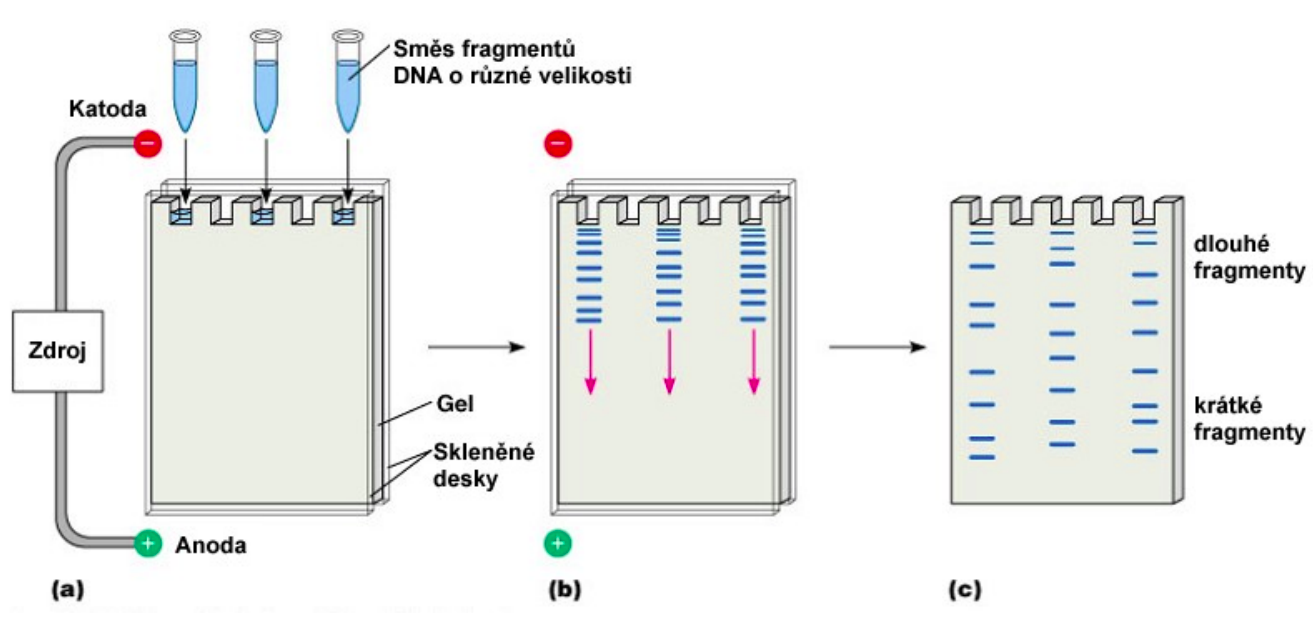
\includegraphics[width=\textwidth]{./img/elektroforeza.png}
		\caption{Elektroforéza. \cite{elektroforeza_img}}
		\label{fig:elektroforeza}
\end{figure}



 Mezi hlavní metodu patří sanger sekvenování oproti jiným je pomalé a spíše se používá k porovnání s novějšími metodamy. 
TODO možná sem ještě přidat obrázek tý destičky.. ale zatím se nenašla nějakej hezkej.

U Kir jsou 2 hlavní typy haplotyp A a B, které jsou definovány typem a počtem specifických KIR genů. Neexistuje žádné jednoduché univerzální kriterium definující a odlišující tyto haplotypy. 


 
 
\section{NGS next-generation sekvenování}
Next-generation sekvenování někdy označováno jako metody druhé generace. V porovnání se Sangerovo sekvenování jsou tyto metody rychlejší a levnější. NGS metody jsou schopné detakovaat přidávání bází jednu po druhé a zároveň  


Někdy označováno jako metody druhé generace
 
jsou schopny detekovat přídávání bází jednu po druhé a zároven sekvenovat tisíce až miliony rozdílných molekul DNA na jednou. 

hlavní nevýhodou oproti saner je krátká maximální délka výsledních sekvencí. od 100 až po 500 bází (sanger nabízí až 1000 bází)
menší přesnost a častější chyby
nejdřívé nastříhané na malé krátké části na konec přilepen adaptér - velmi krátká molekula DNA o přesně dané sekvenci
- slouží k následnému navázání sekvenovaného úseku na pevných povrch. Takto upravené DNA se říká sekvenační knihovna
po uchycení pomocí adaptéru je každý řetězec DNA namnožen čímž vznikne klastr identických molekul DNA koncentrovaných v jednom místě
tato koncentrace posílí výsledný signál zachycený kamerou neboť signál z pouhé jedné molekuly DNA by nebyl dostatečně silný
 
Je rychlé a relativné nenáročné zprácování jednotlivých vzorků. Tisíce až miliony sekvencí mohou být produkovány během jednoho sekvenčního procesu. K popularitě této metody nepomohla i komerciaze cenově dostupních stolních sekvenátorů.


\subsection{454 sekvenování a Ion Torrent}
454 bylo vypuštěno do světa v roce 2005. Dokáže analyzovat více než milion molekul DNA najednou a délka každé jednotlivé sekvence se pohybuje okolo 700 až 1000 bází.
\\
\\
V prvním kroku sekvenování je molekula DNA přichycena na malou "kuličku" na jejimž povrchu se postupně namnoží až kuličku zcela pokryjí identické molekuly DNA. Následuje vložení kuličky i s DNA do jedné z milionů komůrek na destičce s reakční směsí. V určitém momentě je do této směsy přidán vždy jen jeden typ báze. Mezi jednotlivými fázemi přidávání určité báze jsou přebytečné nukleotidy z předešlého kroku odstraněny. To znamená že v reakční směsy je vždy jen jeden typ nukleotidů. Během vložení každé nové báze do rostoucího řetězce DNA je uvolněna molekula zvaná pyrofosfát.  Tento pyrofosfát se následně spustí několik chemických reakci. V poslední fází enzym luciferáza vydá světelný záblesk, který je možné zachytit citlivou kamerou.  Tento postup se nazývá pyrosekvenování. V případě kdy je do řetězce přidáno několik stejných bází za sebou, například gen obsahuje podřetězec AAA, je vyzářeno , v našem případě, třikrát více světla než v případě jedné přiřazené báze. Kamera snímá celou destičku a na základě. která komůrka se rozsvítí pozná kde přoběhlo přidání báze. Intenzita světla pak určuje kolik bází bylo přidáno na jednou. 
\\
\\
Sekvenování Ion Torrent funguje na podobné princupu sekvenování s rozdílem, že místo světla se měří změna pH v reakční směsy. Podle intenzity změny pH pak pozná kolik nukleotidů bylo přidáno do rostoucího řetězce.
\\
\\
Hlavní slabinou těchto dvou metod je značná chybovost při přidání mnoha stejných nukleotidů do řetězce za sebou. Například pří přidání 10 A, nebude odpověď jednoznačná zda je to 10 A nebo 9.


\subsection{Illumina}
Při sekvenování pomocí Illumina jsou páry dvoušrobovice rozděleny na dva řetězce. Jednotlivé řetezce jsou následně přichyceny na malou destičku pomocí adaptéru. Každý řetězec se následně opakovaně množí až na destičce vznikne několik shluků. Přidání jedné molekuly ke druhé probíhá obdobně jako u Sanger sekvenování. Každý shluk tvoří jednu skupinu vzájemně identických řetězců. Mezi volné nukleotidy jsou opět zahrnuty nukleotidy označená fluorescenční barvou za které nelze nic navázat. Oproti sangerovu sekvenování je ale tato blokace vratná a po přečtení citlivou kaměrou dojde k odstranění blukující části molekuly. Počítač si pak následně zpětně spočítá co to bylo za barvu (nukleotid.) 
Nejčastější chybou je špatně určené písmenko
  


Dokáže sekvenovat až 900 miliard? bází najednou. 
potřebuje kratší sekvence - stovky bází



Je tam hezká tabulka porovnání tak by se sem mohla taky dát

\subsection{SOLiD}
SOLiD (Sequencing by Oligonucleotide Ligation and Detection)
narozdíl od předchozích nespolehá na enzym DNA polymerázu,ale na enzym ligáza, který umí připojit části jednořetězcových molekul DNA k stávajícím řětězcům DNA.

 Zjednodušeně lze říci,
že při SOLiD sekvenování se k templátu
přidají kousky DNA, tzv. sondy, které za -
čínají všemi možnými dvojkombinacemi
čtyř základních nukleotidů, tedy 16 různých sond. Každá sonda také nese jednu ze
čtyř fluorescenčních značení, což znamená, že čtyři různé dvojkombinace nukleotidů jsou označeny stejnou fluorescenční
značkou. V každém kroku pak enzym ligáza připojí k rostoucímu novému řetězci
sondu nesoucí dvojkombinaci nukleotidů odpovídající templátové DNA a snímač
přečte její fluorescenční značení, které je
poté odstraněno a může se připojit další
sonda. Aby došlo k přečtení kompletní sek -
vence, je jedna templátová molekula čtena
opakovaně, ale „začátek“ čtení se vždy
posune o jeden nukleotid, a každá báze je
tak přečtena několikrát. Z kombinace znalosti sekvence adaptéru, kterým sekvenovaná DNA začíná, a výsledného signálu
čtyř fluorescenčních barev, jak jdou po
sobě v jednotlivých čteních, lze odvodit
výslednou DNA sekvenci. SOLiD sekveno -
vání má podobný výstup jako Illumina
a produkuje rovněž krátké sekvence (maximálně 100 bází). SOLiD má problémy se
čtením palindromatických úseků (sekvencí shodných u obou komplementárních ře -
tězců), jež mohou vytvářet smyčku v templátové DNA, která je pak nepřístupná pro
nasednutí 

\section{Metody třetí generace}
Narozdíl od drohé generace není DNA templat před sekvenováním nijak namnožen a tak je čten jen z jediné původní molekuly.

Například PacBio od Pacific Bioscience
k detekci sekvence také využívá fluoresenčně značené nukleotidy. 
vysoká citlivost umožňuje v reálném čase zaznamenávat zařazení byť jediného nukleotidu do jediného řětězce DNA.

Oxford Nanopore
 Zde je jednořetězcová molekula DNA protahována mikroskopickým pórem na syntetické membráně.
Protože každá DNA báze má trochu jiný
tvar, dochází při protahování k odlišnému
„ucpání“ póru a citlivé snímače přístroje
dokážou zjistit, jak výrazně je pór v danou
chvíli „zaplněn“, a tedy jaká báze v daný
okamžik membránou prochází.
výhoda je velikost .. je to malý kapesní přístroj který se dá přes USB přípojit k počítači. 

obě jsou schopné přečíst 10 i více tisíc bází v rámci jedné analyzované molekuly DNA a 

vysoká frekvence chyb 10-15 procent

sekvenování celého genomu pomocí sangerova metody stálo několik miliard dolarů a trvalo zhruba 10 let.
dnes by to stálo zhruba desítky tisíc dolarů 

největší problém u sekvenování je že jsou roztříhané na malé části a pak je musíme zpět poskládávat zpět.


zajímavost

Další metodou, která se dočkala rozmachu díky sekvenování druhé generace, je
sekvenování transkriptomů (viz Živa 2016,
2: 61–63 a 3: 104–106). Při této metodě se
místo kompletního genomu zjišťuje sek -
vence pouze aktivních genů, tedy genů,
které jsou v buňkách v danou chvíli přepisovány do mediátorové RNA (mRNA)
a překládány do proteinů. Při sekvenování
transkriptomů se nejdříve získá veškerá
mRNA z daného organismu (nebo jen z urči -
té tkáně, orgánu apod.) a přepíše se do DNA
molekuly zvané copy DNA (cDNA). Teprve
tato DNA je následně sekvenována. Výhoda sekvenace transkriptomů oproti celým
genomům spočívá v získání sekvencí genů
bez balastní (nepotřebné) nekódující části
genomové DNA. Nekódující DNA totiž často tvoří podstatnou část genomu organismu a sekvence jednotlivých genů je proto
potřeba v této záplavě pracně hledat, což
se ne vždy spolehlivě daří. 


Pomocí sekvenování transkriptomů také
můžeme studovat odlišnou expresi (míru
přepisu) jednotlivých genů v závislosti na
vnějších nebo vnitřních podmínkách. Zpravidla porovnáváme transkriptomy získané z organismu nacházejícího se ve dvou
či více různých „stavech“ – např. pěstova -
ného při různých teplotách nebo ve zdravém či nemocném stavu apod. Porovnáním
přítomnosti a četnosti sekvencí jednotlivých genů lze určit, které geny jsou v příslušné „fázi“ aktivnější, a tedy nejspíše
zodpovídají za reakci daného organismu
na tento „stav“, třeba na změnu teploty
nebo onemocní.


Další novinkou vzešlou z dílny sekveno -
vání druhé generace je sekvenování „exomu“. Místo celého genomu nebo v danou
chvíli aktivních genů (transkriptomů) sek -
venujeme pouze kódující část genomu,
tedy geny jako takové, bez intronů (Pozn.:
U většiny eukaryotických organismů se
většina genů skládá z exonů a intronů.
Exony představují kódující část genu, za -
tímco introny nic nekódují, a proto jsou
před přeložením do patřičného genového
produktu vystřiženy.). Samozřejmě předem potřebujeme velmi dobře znát genom
daného organismu a hranice jednotlvých.


kódujících částí příslušných genů. Tato
metoda se často používá při klinických
studiích některých geneticky podmíněných chorob. V takovém případě lze po -
rovnat exomy jedinců trpících poruchou
a jedinců zdravých, a následně tak identifikovat mutace, které jsou pravděpodobně zodpovědné za nástup nemoci. Právě
cenová dostupnost a vysoká efektivita
metod sekvenování druhé generace dnes
umožňuje zkoumat a rozpoznat příčiny
řady vzácných a dříve málo studovaných
genetických poruch.
\section{Read}
In DNA sequencing, a read is an inferred sequence of base pairs (or base pair probabilities) corresponding to all or part of a single DNA fragment. A typical sequencing experiment involves fragmentation of the genome into millions of molecules, which are size-selected and ligated to adapters. The set of fragments is referred to as a sequencing library, which is sequenced to produce a set of reads. Je to z wiki zase
\\
\\
V DNA sekvenování, read je odvozená sekvece párů bází odpovídající celému fragmentu DNA nebo jeho části
To znamená že read je kus DNA který by mohl odpovídat nějakého konkrétnímu genu? 
\\
\\
Pak tam ještě bylo psaný něco o read lenght
Sekvenační technologie se liší? v délce vyrobenybch readů. 
Ready díkjy 20-40 párů bází (bp) jsou ultrakrátké
Typická sekvenační metoda vytváří ready délky 100 až 500 bp

Sekvenančí platforma (Illumina) - podle toho se pak připravuje ta sekvenační knihovna


DNA knihovny - podle wikiskripta

DNA knihovny jsou kolekce klonovaných DNA fragmentů genomu určitého organismu (cDNA), které jsou skladovány uvnitř hostitelských organismů (zejména bakterií). cDNA (copy DNA, complementary DNA) je získávána přepisem z mRNA pomocí enzymu reverzní transkriptázy.

Kvalita knihovny
Při přípravě sekvenční knihovny je důležité získat co nejvyšší úroveň složitosti. Jinými slovy, je důležité, aby konečná knihovna co nejvíce odrážela jedinečnost výchozího materiálu. Tento výsledek lze získat především omezením počtu segmentových duplikací. Čím kratší jsou fragmenty, tím vyšší je pravděpodobnost, že jsou fragmenty méně specifické a mohou se zarovnat na více než jednom lokusu referenční sekvence. Složitost knihovny lze tedy v podstatě měřit procentem duplicitních čtení, které jsou přítomny v sekvenčních datech

READY - zase wikipedie
In DNA sequencing, a read is an inferred sequence of base pairs (or base pair probabilities) corresponding to all or part of a single DNA fragment. A typical sequencing experiment involves fragmentation of the genome into millions of molecules, which are size-selected and ligated to adapters. The set of fragments is referred to as a sequencing library, which is sequenced to produce a set of reads

Sekvenování mRNA s použitıím NGS technologií umožňuje měření genové exprese celého
transkriptomu. Postup a provedení RNA-seq experimentu je znázorněn na obr. 14.
Prvním úkolem je vyčistit zkoumaný vzorek o rRNA, tRNA a mitochondriální RNA,
které u prokaryot i eukaryot tvoří přibližně 75 procent všech RNA molekul. Navzdory použití
purifikačních metod, mezi které patří například poly(A)purifikace a DNS normalizace,
sekvenační data mohou obsahovat menší množství těchto RNA molekul [59]. Ty mo-
hou být odfiltrovány v následujícíh krocích bioinformatickými postupy. Zbylá mRNA
je poté nastříhána na menší části, a je z ní připravena knihovna krátkých fragmentů s
navázanými adaptory. Ty jsou poté sekvenovány sekvenačním přístrojem a jako výsledek
získáme tzv. ready. Anglické slovo ’read’ značí datovou reprezentaci krátké sekvence
DNA obvykle 50-150 bp dlouhou, která byla vyprodukována sekvenačním přístrojem.
Samotné ready však nemají žádnou vypovídající hodnotu, a proto jsou dále bioinformat-
icky zpracovány. Namapováním na referenční sekvenci zjistíme jejich genomickou pozici,
ze které byly odvozeny. Většina readů je namapována na exony, což jsou transkripčně
aktivní jednotky, a pouze malé množství readů je namapováno na transposony. Ready
které nejde namapovat v celku, jsou rozděleny na menší části a ty jsou namapovávány
zvlášť. Rozdělené ready umožňují jednodušší identifikaci mezer mezi exony (angl. splice
junctions)
tohle je z tý diplomky single-pair
\section{Bordel}
SANGER
Vybraná sekvence se vloží do reakční směsi s radioaktivně označným primer  

Během procesu replikace jsou řetězce rozděleniny na dvě vlákna. 
V praxi to není tak snadné a hrají roly i další proteiny. 
Mezi nukleotydi plavou i uprvené nukleotidy které nesou specifickou fluorescenční barvu a za ně už neni možné aby s něco nevázalo.  Podle barvy poznáme o jakou bázi se jedná. 
Náhodný přerušováním syntézy vznikají různě dlouhé molekuly. 

výhody dlouhá délka sekvencí které se dají sekvenovat jedinou reakci a vysoká přenost čtení
v rámci celého procesu dochází k sekvenování pouze jednoho úseku DNA 
vysoká cena a nízká rychlost
 K sekvenaci se použtívá gelová elektrofézy
 použitelná k sekvenování krátké sekvence jednovláknové DNA. 
 využívá biologického procesu replikace DNA
 Vybraná sekvence se vloží do reakční směsi s radioaktivně označným primer
 rozdělí se to na přibližně 
 namnoží se to .. 
 pak se to hodí do něčeho co nakonci svítí tak ty se navážou na příslušnej konec.. 
 pak to pustíme do gelu .. 
 nejkratší projedou nejdál
 nejdelší zůstanou co nejblíž a podle toho pak sestavuju jak ta sekvence vypadá
Sekvenování DNA je souhrný termín pro biochemické metody, jímiž se zjišťuje pořadí nukleových bází (A, C, G, T) v sekvencí DNA. Tyto sekvence jsou součástí dědičné informace v jádru.
Adenin s thyminem a cytosins s guaninem.

zjišťvání přímární struktury nukleových kyselin (sekvencování)
Někdy se sekvenují pouze jisté části genomu které mají pro výzkumníka v daném okamžiku význam.
Užitečné nejen ve výzkumu ale i v diagnostice nemocí či forenzní medicíně. 


454 
, kde probíhá sekvenační reakce na principu pyrosekvenování.  

 Pyrosekvenování se za -
kládá na skutečnosti, že během vložení
každé nové báze do rostoucího řetězce
DNA se uvolní molekula zvaná pyrofosfát
(proto pyrosekvenování). Uvolněný pyrofosfát se posléze stane součástí několika
na sebe navazujících enzymatických reakcí, na jejichž konci čeká enzym luciferáza
Ten vydá světelný záblesk, jenž lze za -
chytit vysoce citlivou kamerou


 Při 454 sek -
venování je v určitém momentě přidán do
reakční směsi vždy pouze jeden typ báze
a v okamžiku, kdy je tato báze vložena do
rostoucího řetězce DNA, dojde přes uvolněný pyrofosfát a luciferázu ke světelnému
záblesku. Pokud je do rostoucího řetězce
DNA zařazeno několik stejných bází za se -
bou, např. když DNA molekula templátu
obsahuje sekvenci AAA a je tedy přidáno
třikrát T, vyzáří se třikrát více světla než
v případě přiřazení jednoho T

. Kamera
snímá celou destičku a podle toho, která
komůrka se rozsvítí, pozná, kde proběhlo
přidání báze, a podle intenzity světla ko -
lik bází bylo přidáno najednou

Nukleotidy jsou přidávýny jeden po druhém a mezi jednotlivými dochází k odtranění přebytečných nukleotidů.
takže v rekční směsy je vždy jen jeden typ nukleotidů.


Ion Torrent je na podobném principu jako pyrosekvenování
ale neměří světlo ale změnu pH v reakční směsy. Pod
podle intenzity změny pH

protože spolehají na sílu signálu aby věděli kolik bází bylo přidáno  nejednou mají obě metody problém se čtením dělších řetězců obsahující práce jen jednu bázi například AAAAA. nebude jednoznačná odpověď zda je to 9 A nebo 10.

Ilumina
Dokáže sekvenovat až 900 miliard? bází najednou. 
potřebuje kratší sekvence - stovky bází
pomocí adaptéru přichyceny molekuly DNA na malou destičku

Každá molekula DNA se pak opakovaně namnoží, až na destičce vznikne
mozaika milionů klastrů, přičemž každou
skupinu tvoří vzájemně identické molekuly. Vlastní sekvenační proces pak využí -
vá podobného mechanismu jako Sange -
rovo sekvenování, kdy jsou do rostoucího
řetězce zařazeny báze s navázanou fluorescenční barvou (každé písmeno má speci -
fickou barvu), které syntézu zastaví.

tato blokace je orpoti sangerovi vratná
 popřečtení citlivou kamerou dojde k odstranění fluorescenčního značení i blokující části molekuly
 a může se pokračovat
 
 kamera snímá celou destičku
 a podle rozdílné fluorescence pozná co bylo přidáno u každého z milionů skupin
 
 počítač si to pak zpětně přechroupa krok po kroku.
 

nejčatější chybou je špatně přečtené písmenko. 
jinak má 99 procentní úspěšnost

\chapter{Analyza dostupných bioinformatických nástrojů pro zpracování NGS dat}
\section{Referenční genomy}
Referenční geny byli převzaty z http://www.ebi.ac.uk/ipd/kir/
All files in this folder are provided in the FASTA sequence format. Please note the FASTA format contains no alignment information.

Files designated “X\_prot.fasta”, where X is a locus or gene, contain protein sequences. Please note that alleles that contain non-coding variations may be identical at the protein level. 

Files designated “X\_nuc.fasta”, where X is a locus or gene, contain the nucleotide coding sequences (CDS). Please note that alleles that contain non-coding variations may be identical at the CDS level.

Files designated “X\_gen.fasta”, where X is a locus or gene, contain genomic DNA sequences. Please note for alleles that do not possess genomic sequences, there will be no entry in the file.

\section{ART}
ART (next-generation sequencing read simulator) je sada simulačních nástrojů, které generují syntetické ready, jako kdyby byli získány sekvenováním pomocí NGS. Nástroj ART dokáže simulovat ready ze sekvenátorů Illuminas, 454 společnosti Roch a SOLid od společnosti Applied biosystém. Ready, vytvořené nástrojem ART jsou používány pro testování a analýzů nástrojů zpracovávající právě NGS sekvence jako například zarovávání (nástroj Bowtie). 
\\
\\
ART je implementován v jazyce C++ a je dostupný s licencí GPL verze~3 pro operační systémy Linux, MacOs a Windows. Je možné ho použít i jako C++ package. Pro jeho spuštění je nutní mít nainstalovaný compilator GNU g++ 4.0 nebo vyšší a knihovnu GNU gsl. 
\\
\\
Data získána z FN Plzeň byla sekvenována nástrojem Illuminas proto i syntetické ready budou simulovat tento sekvenátor.    
 Výstupy se čtou ve formátu FASTQ a zarovnání ve formátu ALN. může generovat zarovánávání také ve formátu SAM nebo UCS BED. \cite{art}

\subsection{pokus to nejak spustit}
Takze kdyz otebru hlavni readme tak mi to riká že tam jsou read me pro jednotlivy verze sekvenatoru .. jako je ilumina , 454 a solid.
A píšou že by měl mít človek GNU g++ 4.0 nebo above (to je vyšši ne)
A GNU gsl library

pak se to musí skompilovat 

./configure --prefix=\$HOME
	       	make
	       	make install	 
	 
teď mě zajímá ta ilumia tak podle readme ilumina tak můžu vlést do složky examples a tam pustit skript run\_test\_examples\_illumina.sh , tak tam jsou 4 příklady použití 
a pokud asi všechno dobře porběhne tak se mi zobrazí pár nových souborů ve složce examples.. 

FASTQ - *.fq data file s ready. pro paired-red simulator
*1.fq obsahuje data pro rvní ready a *2.fq rdu druhy ready

tohle nějak funguje
MSv3 tam musím dát abych to mohla dostat na délku reafu 250 a p znaci ze to je paired.. 
% art_illumina -ss MSv3 -sam -i amplicon_reference.fa -p -l 250 -f 10 -m 300 -s 10 -o moje_art_data


\subsection{FASTQ}
Sekvenační přístroje produkují data ve formátu FASTQ takže i ART musí logicky generovat tenhle formát.
Pokud jsou ready v páru tak je na konci .1
a druhý read z páru tam má .2 to jsem u těch svých přímo nenašla 

ale máš teda tři druhy single end, paired-end a matepair. 

FASTQ obsahuje obě základy sekvence ?? both sequence bases a kvality skore je to v následujícím formátu
@read\_id
sequence read
+
base quality scores je kódovany by ascii code of a single character, kde je kvalita rovná score to ascii code character minus 33. chápu proč tam je to -33 protže když se podíváš do asci tabulky tak je tam od 33 první normální znak jinakjsou tam divný .. 
takže třeba otazník je v asci na 63 takže -33 takže má ohodnocení kvality 30
jen by mě teda zajímalo v jakým sme intervalu? - je 45 v asci a nevím jestli to je teda od 0 do 100?  a teda nejvyšší číslo znamená nejkvalitnější a nejmenši míň kvalitní? Podle tý diplomky to tak je že čím vyšší číslo tím kvalitnější a většinou je to od 0 do 40 jen zřídka to překročí hodnotu 60, když je tam 10 tak to znamneá že jedna báze z deset je špatně.. když je tam 30 tak to znamená že jedna z 1000 je špatně.
já tam mám třeba F a to je 70.

example:
		@refid-4028550-1 
		caacgccactcagcaatgatcggtttattcacgat...
		+ 
%		????????????7?????<??>??=&?<<?-<?0?...

ALN - zarovnání readů
zase *1.aln pro první a *2.aln pro druhý
soubor je rozdělen na hlavičku a body část
obsahuje hlavičku a v tý hlavičce je jakým příkazem byl soubor vygenerován a reference na sequnce id a jejich délku
@CM tag pro příkaz a
@SQ pro reference sequence
Hlavička vždycky začíná s 
%##ART a končí s ##header end

		HEADER EXAMPLE

%		##ART_Illumina  read_length     35
%		@CM     ../art_illumina -i ./testSeq.fa -o ./single_end_com -l 35 -f 10 -sam -rs 177
%		@SQ     seq1    7207
%	       	@SQ     seq2    3056
%		##Header End
		
v body jsou všechny zarovnání 
%		>ref_seq_id	read_id	aln_start_pos	ref_seq_strand
%	       	ref_seq_aligned
%	       	read_seq_aligned 
	    
	    aln\_start\_pos označuje počáteční pozicí v referenci sekvence, je vždy relativní vzhledem k vláknu referenční sekvence
	    To znamená že aln\_start\_pos plus (10) vlákno je odlišný od  aln\_start\_pos minus (-) vlákna.. ???? WHAT???
	    
		ref\_seq\_aligned je zarovnaná oblast referenční sekvence, která může být plus vlákno nebo mínos vlákno referenční sekvence
		ref\_seq\_aligned je zarovanný read, který je vždy ve stejné orientaci jako stejný read v odpovívajícím fastq suboru.  
		
		
			    
	    
	       	
		aln\_start\_pos is the alignment start position of reference sequence. aln\_start\_pos is always relative to the strand of reference sequence. That is, aln\_start\_pos 10 in the plus (+) strand is different from aln\_start\_pos 10 in the minus (‐) stand.  
	
		ref\_seq\_aligned is the aligned region of reference sequence, which can be from plus strand or minus strand of the reference sequence. 
		read\_seq\_aligned is the aligned sequence read, which always in the same orientation of the same read in the corresponding fastq file. 

SAM je standardní formát pro NG sekvence ready zarování
BED o tom tam nic neni jen 
NOTE: both ALN and BED format files use 0-based coordinate system while SAM format uses 1-based coordinate system.

pak jsou tady 4 doporučené použití
$art_illumina [options] -ss <sequencing_system> -sam -i <seq_ref_file> -l <read_length> -f <fold_coverage> -o <outfile_prefix>$
$art_illumina [options] -ss <sequencing_system> -sam -i <seq_ref_file> -l <read_length> -c <num_reads_per_sequence> -o <outfile_prefix>$
$art_illumina [options] -ss <sequencing_system> -sam -i <seq_ref_file> -l <read_length> -f <fold_coverage> -m <mean_fragsize> -s <std_fragsize> -o <outfile_prefix>$
$art_illumina [options] -ss <sequencing_system> -sam -i <seq_ref_file> -l <read_length> -c <num_reads_per_sequence> -m <mean_fragsize> -s <std_fragsize> -o <outfile_prefix>$

pak tam máš parametry 

a jak dlouhý chceme simulovat ready? 



\subsection{bordel}
ART is freely available to public. The binary packages of ART are available for three major operating systems: Linux, Macintosh, and Windows. ART is also available as Platform-independent C++ source packages. Each package includes programs, documents and usage examples.

ART simuluje ready napodobobáním skutečných procesů sekvenování s empirickým chybovým modelem nebo quality profiles summarized from large recalibrated sequencing data
ART může také simlovat čtené pomocí uživatelského vlastního read arror modelu nebo quality profiles

TODO - tohle úplně nechápu ART podporuje simulaci jedno párových, dvou párovcýh tří hlavních komerčních sekvenčních platfoem 
Výstupy se čtou ve formátu FASQ a zarování ve formátu ALN. 
ART může také generovat zarovnávání ve formátu SAM nebo UCSC BED
ART lze použít společně se simulátory varient genomů VarSim 
\\
to je odtud %https://www.niehs.nih.gov/research/resources/software/biostatistics/art/index.cfm
454 sekvenování je pyrosekvenování, které cycklicky testuje přítomnost každého ze čtyř nukleotidů DNA (T, A, C, G)

SOLid ke kódování 16 různých dinukleotidů používá čtyči fluoresenční barevná barviva, každé barvivo kóduje čtyři dinukleotidy
 


tak jsem stáhla normálně nejnovější verzi z niehs.nih.gov a podle instrukcí co byli v souboru INSTAL dala % ./configure && make && make install


musí se brát v potaz že z toho generátoru nikdy nebudou data taková jako reálná.. realná budou horší 




\section{Bowtie}
Bowtie je rychlý a paměťové efektivní nástroj pro zarovnávání krátkých sekvencí DNA na velké genomy. Indexace pomocí Burrows-Wheelere transformace dovoluje zarovnávání více než 25 milionů readů za CPU hodinu pro lidský genom s pamětí příblížně 1.3 gigabajtů. Bowtie přidáváa k Burrows-Wheeler technice backtracking algoritmus pro sledování nekonzistence. ??


\subsection{Bordel}
Bowtie je napsanej v c++ a používá knihovnu seqAn

Na lidském genomu je nástoj Bowtie v porovnání s nástoji Maq a SOAP rychlejší. 
Citlovost má bowtie srovnatelné s nástojem SOAP a o něco menší než Maq. Ale je možnost pomocí příkazové řádky zvýšit citlivost na úkor rychlosti běhu progamu.
Oproti SOAP bowtie potřebuje méně paměti 1.3 GB RAM. 
Bowtie zarovnává  25 milionů readů za hodinu. může běžet paralelně.

indexi vytváří permanentní a lze je použít napříč běhy 
pro lidský genom je to 2.2 GB takže ho lze distribuovat přes internet
rychlost a malá paměť způsobuje především Burrows wheeler v kombinaci s backtrackingem.

Podrporuje standardní vstupní formáty FASQ a FASTA.

Bowtie je open source.

 
na stránkách elixir-europe což je oragnizace co má dávat dohromady všechny vědecký veci a bla bla.



Tak tam je přímo Bowtie \cite{bowtie}

\subsection{Bowtie 2}
Note that SOAP2 and Bowtie do not permit gapped alignment of unpaired reads.
 memory footprint of Bowtie 2 (3.24 gigabytes)
 Bowtie 2 by mělo být vhodnější pro delší ready než Bowtie1.
 We extracted a random subset of 1 million reads from each and aligned them with BWA-SW and Bowtie 2. We did not align with Bowtie, BWA or SOAP2 because those tools are designed for shorter reads.
Bowtie už je překonanej nejenom Bowtie2 ale i BWA.
Bowtie2 je podle studie znatelně lepší než Bowtie, SOAP2.
tyhle výsledky jsou na syntetických readech

vypadá to že bowtie 2 už nepoužívá tamten index ale používá nějaký Full-text minute index–assisted search což vypadá že je kombinace burrows wheelera a ještě něčeho.
We found that Bowtie 2, a method that combines the advantages of the full-text minute index and SIMD dynamic programming, achieved very fast and memory-efficient gapped alignment of sequencing reads

je zase open source
\cite{bowtie2}


šla jsem přes docker docker image ls - zobrazi vsechny image pak docker run a ID image
sudo docker run -i -t 3c2b9a287f82 /bin/bash
sudo docker ps -a

Tak jsem nakonec žádnej docker nepotřebovala a stáhla jsem to tady %http://bowtie-bio.sourceforge.net/tutorial.shtml
 po kliknuti na bowtie binary release.

na strance 25.4 je řečeno o hledání tch nejlepších zarovnání a je tam možnost --best ale že je dvakrát nebo třikrát pomalejší než normální mod.. a jde o to že najde první přijatelný a to označní kdežto při tom best prohledá co nejvíc a hledá to nejlepší i mezi těma přijatelnýma a to je pomalý.

takže zarovnání by mohlo být teoreticky namapování na referenční gen???

\subsection{bordel}
tak jsem  to stáhla dala do složky a musela jsem teda nastavit proměnou prostředí 
export BT2\_HOME=$/home/kate/Dokumenty/FAV/Diplomka/existujicisw/bowtie2-2.4.1-linux-x86_64/$
pak jsem pustila tohle: 
\$BT2\_HOME/bowtie2-build \$ $BT2_HOME/example/reference/lambda_virus.fa lambda_virus$
a nakonec se mi vytvořili nějaký nový soubory lambda virus 1 atd.. v tom bowtie 2 adresáři

dělala jsemt o podle tohohle webovky %http://bowtie-bio.sourceforge.net/bowtie2/manual.shtml#getting-started-with-bowtie-2-lambda-phage-example


z bowtie pak teda leze asi SAM formát

\subsubsection{SAM}
1. název readu který je zarovnáván

2. Sum of all applicable flags. Flags relevant to Bowtie are:
součet všechn aplikovaných (příslušných flags). Flagy relevantní k bowtie jsou: 
1 - read je jeden z páru
2 - zarovnání je one z paired proper (The alignment is one end of a proper paired-end alignment)
4 - read má reported alignments
8 - read je jeden z páru a má reportovaný zarovnání
16 - zarování je obrácená reference vlákna
32 - The other mate in the paired-end alignment is aligned to the reverse reference strand
64 - read je mate 1 in a pair
128 - read je mate 2 in a pair

Thus, an unpaired read that aligns to the reverse reference strand will have flag 16. A paired-end read that aligns and is the first mate in the pair will have flag 83 (= 64 + 16 + 2 + 1).

3. jméno referecnce ze které zarování patří
4. 1-based offset into the forward reference strand where leftmost character of the alignment occurs 1-based odszaneí v následující referenci 
5. kvalita mapování
6. CIGAR reprezentace zarovnání
7. název reference kde je zarovnán kamarád 
8. 1-based zarování ofsetu k nálsedující refenrenci 
9. Odvozená délka fragmentu. Velikost v závoru je že se mate nachází předtím. 0 že jsem nezarovnali mate
10. read sekvence
11. ASCII encoded read kvalita, stejné jako u FASTQ
12. optional pole


SAM Sequence Alignment Map format), respektive jeho binárně
komprimovaná verze BAM (z angl. Binary Alignment Map format).

nakonec jsem to pustila přes IGV ale stejně se tam museli ty indexi dodělat
%java --module-path=lib -Xmx4g @igv.args --module=org.igv/org.broad.igv.ui.Main


% 
% PRO ANGLICKOU SAZBU JE NUTNÉ ZMĚNIT
% CITAČNÍ STYL!
%
\nocite{*}
\bibliographystyle{csplainnatkiv}
{\raggedright\small
\bibliography{literatura}
}

\end{document}
